\documentclass{article}

\usepackage{pgfplots} %http://www.ctan.org/pkg/pgfplots
\pgfplotsset{compat=newest, set layers=standard}

\usepgfplotslibrary{fillbetween}
\usetikzlibrary{intersections}

\title{Numerical Integration}
\begin{document}
\def\horzbar{\text{magic}}

  \pagenumbering{gobble}
  \maketitle
  \newpage
  \pagenumbering{arabic}


\section*{Trapeziod method}

\pgfplotsset{
    integral axis/.style={
        axis lines=middle,
        enlarge y limits=upper,
        axis equal image, width=12cm,
        xlabel=$x$, ylabel=$y$,
        ytick=\empty,
        xticklabel style={font=\small, text height=1.5ex, anchor=north},
        samples=100
    },
    integral/.style={
            domain=2:10,
            samples=9
    },
    integral fill/.style={
            integral,
            draw=none, fill=#1,
            on layer=axis background
        },
        integral fill/.default=cyan!10,
        integral line/.style={
            integral,
            very thick,
            draw=#1
        },
        integral line/.default=black
}


\begin{tikzpicture}[
    % The function that is used for all the plots
    declare function={f=x/5-cos(deg(x*1.85))/2+2;}
]
\begin{axis}[
    integral axis,
    ymin=0,
    xmin=0.75, xmax=11.25,
    domain=1.5:10.5,
    xtick={2,...,10},
    xticklabels={$a=x_0$, $x_1$,,,$x_{j-1}$,$x_j$,,$x_{n-1}$,$b=x_n$},
]
% The function
\addplot [very thick, cyan!75!blue] {f} node [anchor=south] {$y=f(x)$};

% The filled area under the approximate integral
\addplot [integral fill=cyan!15] {f} \closedcycle;

% The approximate integral
\addplot [integral line=black] {f};

% The vertical lines between the segments
\addplot [integral, ycomb] {f};

% The highlighted segment
\addplot [integral fill=cyan!35, domain=6:7, samples=2] {f} \closedcycle;
\end{axis}
\end{tikzpicture}

$h = \frac{b-a}{N -1}$

N - number of points

Total area (integral)

$$\int_a^b f(x)dx \approx h\sum_{k=1}^{N} \frac{f(x_{k-1})+f(x_k)}{2}$$

\section*{Simpson's method}

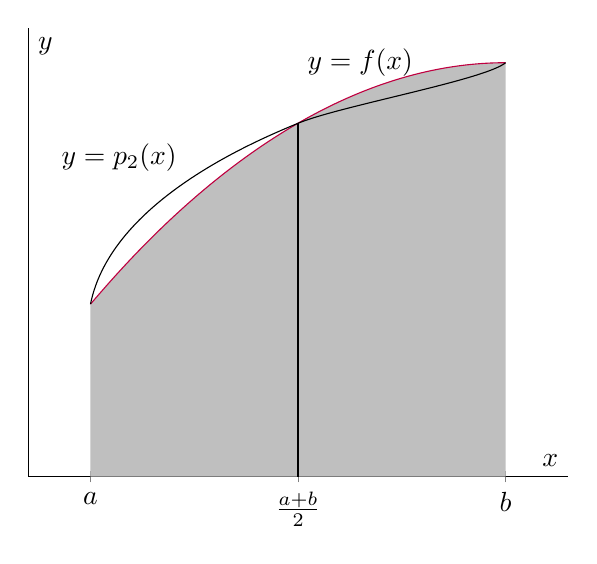
\begin{tikzpicture}
\begin{axis}[axis lines=center, ytick=\empty, 
ymax=1.3, ymin=0, xmax=2.6,xmin=0,
xtick={0.3,1.3,2.3}, xticklabels={$a$,$\frac{a+b}{2}$,$b$},
axis line style={-}, xlabel=$x$, ylabel=$y$]
\draw[name path=A, purple] (2.3,1.2) parabola (0.3,0.5);
\node[] at (1.6,1.2){$y=f(x)$};
\path[name path=B] (\pgfkeysvalueof{/pgfplots/xmin},0) 
                   --(\pgfkeysvalueof{/pgfplots/xmax},0);
\addplot[gray!50] fill between[of=A and B,soft clip={domain=0.3:2.3}];
\draw[name path=C] (1.3,0) -- (1.3,1.025);
\path[name intersections={of=A and C}] coordinate (midpoint) at (intersection-1);
\draw (0.3,0.5) ..controls ++(0.1,0.3) and ++(-0.2,-0.05) .. (midpoint)
                node[pos=0.5,above left]{$y=p_2(x)$} 
                ..controls ++(0.2,0.05) and ++(-0.1,-0.05) .. (2.3,1.2);
\end{axis}
\end{tikzpicture}

$h = \frac{b-a}{2}$

$$\int_a^b f(x)dx \approx \frac{h}{3} \sum_{k=1}^{N/2} \{f(x_{2k-2})+4f(x_{2k-1})+f(x_{2k}))\}$$


\end{document}